\section{Automated plot generation (Stage 2)}
\label{sec:visualizer:plotgeneration}

As a reminder, in stage 2, the visualization system uses the labeled pairwise 
scatter plots to build a classifier and automatically label the rest of the 
plots.

\subsection{Decision tree classification of user interests}
\label{sec:visualizer:plotgeneration:tree}

Given labels for the initialized and actively-selected queries, there are 
several classification models that the visualization system can use to create a 
final fitted model of user interests. One such model is a \textit{decision 
tree}. A decision tree is composed of nodes (which correspond to 
classification labels) and branches (which correspond to decision boundaries). 
A tree is constructed at each node by sampling all $M$ possible vertical and 
horizontal splits in the sample space and selecting the split which minimizes 
the \textit{Gini criterion}~\cite{cutler2010}. A mapping of the sample space to 
a tree is shown in Figure~\ref{fig:visualizer:plotgeneration:tree}. The Gini 
criterion measures the homogeneity of the nodes in each side of the proposed 
split and is computed as follows (for a vertical split)~\cite{cutler2010}:
$$G = N_{\text{left}} \sum\limits_{k\in \{0,1\}} p_{k,\text{left}} 
(1-p_{k,\text{left}}) + N_{\text{right}} 
\sum\limits_{k \in \{0,1\}}  p_{k,\text{right}}(1-p_{k,\text{right}})$$

\noindent where $N_s$ is the number of nodes in side $s$ of a split ($s = 
\{\text{left,right}\}$ in a vertical split, and $s = \{\text{top,bottom}\}$ in 
a horizontal split) and $p_{k,s}$ is the fraction of class label $k$ on side 
$s$ of the split. Note that $k \in \{0,1\}$ in binary classification, which is 
used in the VS. Decision trees are a more sophisticated classification model 
than simple linear regression and retain interpretability. The root node is, 
naturally, the most important as it corresponds to a split that optimizes the 
Gini criterion while the terminal nodes can be thought of as the data's 
homogeneous clusters. However, decision trees are also unstable; perturbing a 
single data point may change the entire tree. Furthermore, due to the nature of 
vertical and horizontal splitting, a single tree cannot fully capture diagonal 
(or non-vertical/horizontal) splits in the decision boundary.

\begin{figure}[htb]
	\begin{center}
		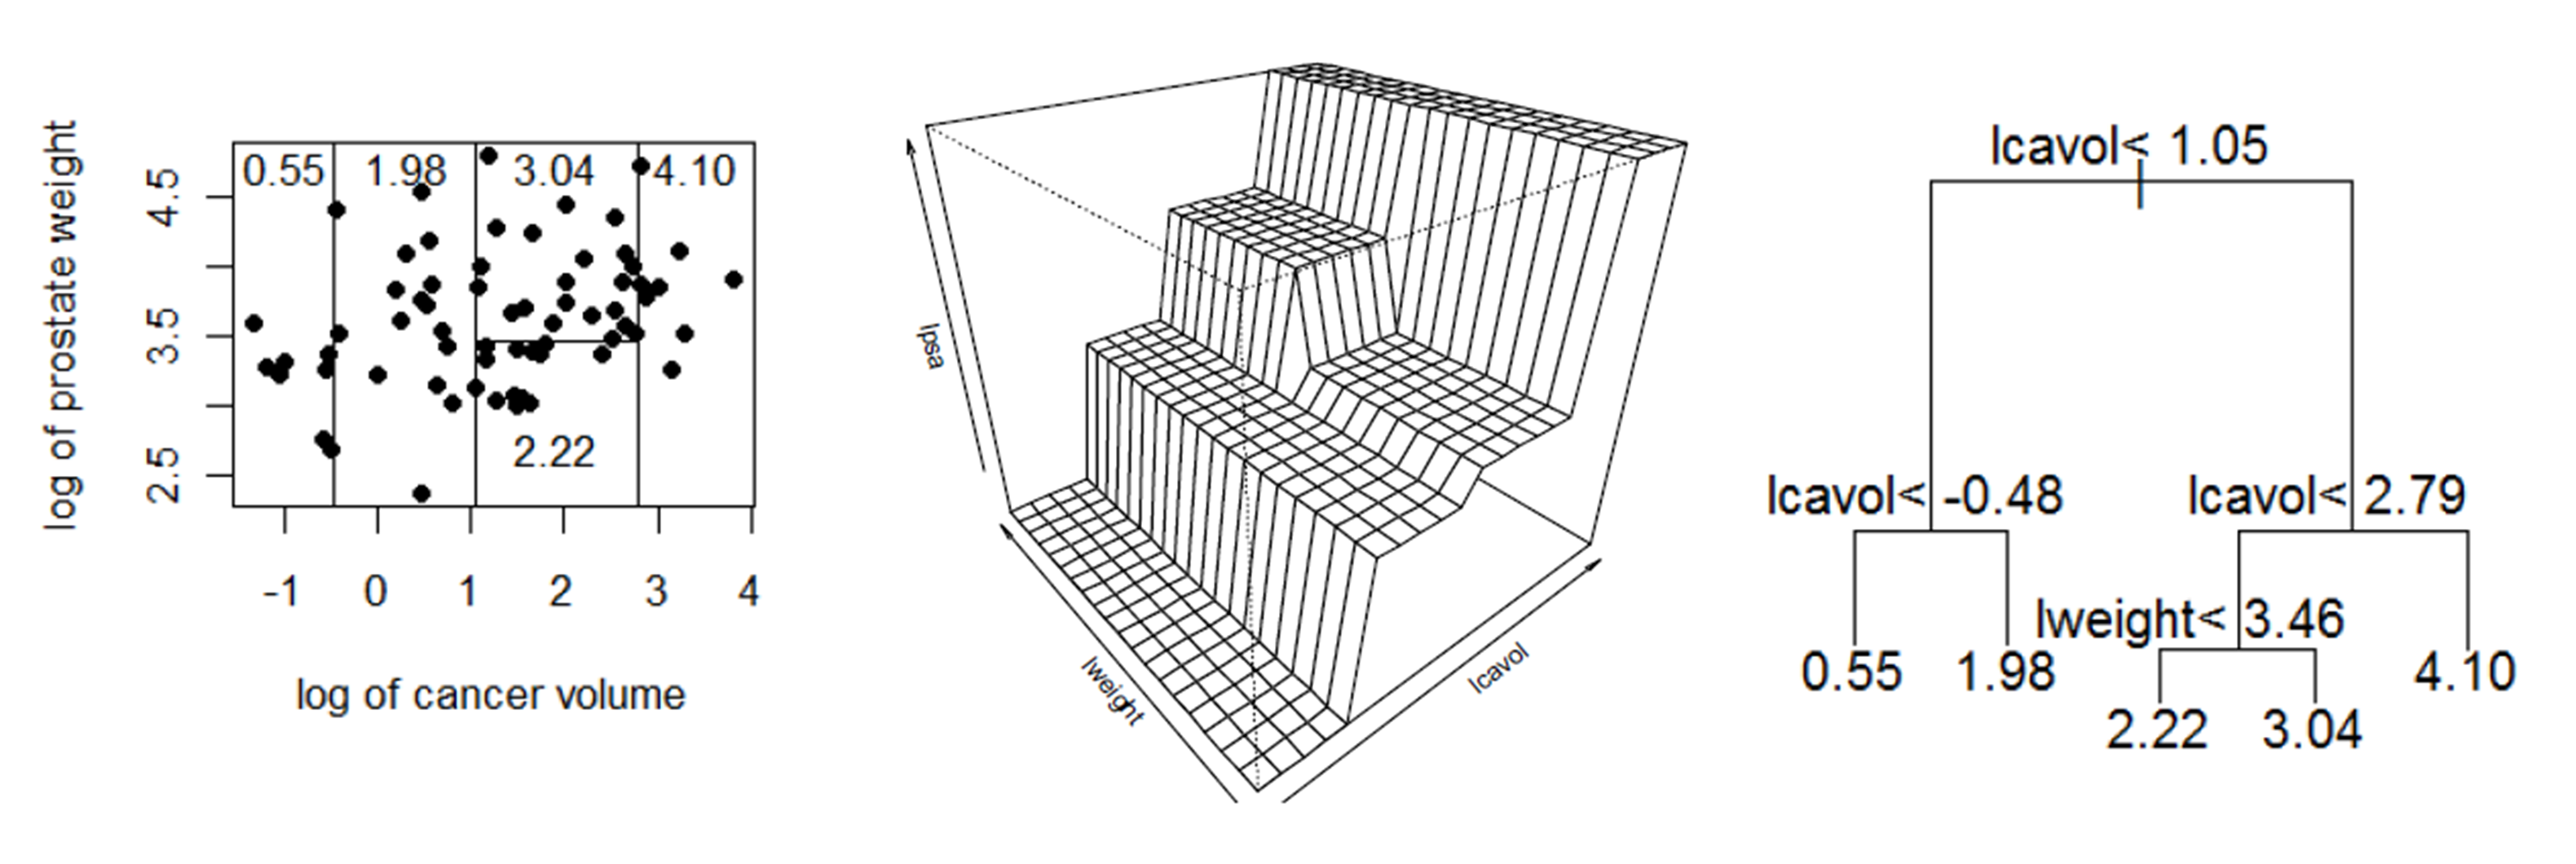
\includegraphics[width=1\linewidth]{ch-visualizer/figures/decisiontree}
		\caption[Mapping the sample space to a decision tree.]{Mapping the 
		sample space (\textit{left}) to a decision tree (\textit{right}). 
		Images from Cutler 2010~\cite{cutler2010}.}
		\label{fig:visualizer:plotgeneration:tree}
	\end{center}
\end{figure}

A \textit{random forest} provides solutions to the problems that a single 
decision tree faces. A forest is composed of many decision trees 
``grown'' from random partitions of the labeled set (the training set). 
Furthermore, each decision tree is constructed by finding the best split among 
$m \in M$ splits~\cite{cutler2010}. This allows each tree to specialize on a 
subset of the data, 
creating a more informative aggregate. A simplistic example of a forest with 2 
trees may be found in Figure~\ref{fig:visualizer:al:tree}. Each tree in the 
forest has a vote of weight one on the label of each unlabeled data point, and 
the forest is aggregated by majority vote, which makes the resulting decision 
boundaries more stable (less variant) on average. On the other hand, a forest 
with many trees is difficult to visualize. However, there are methods to 
simplify a forest into a single tree for the purposes of visualization (rather 
than for usage in classification, as the issue with stability would then 
remain). One such method for single tree approximate is presented by Zhou and 
Hooker~\cite{zhou2016}. Utilization of such a method to present the resulting 
random forest classifier to the user aids in user interpretability of the 
system output while maintaining the robustness of a forest in practice. 
As such, the main stage 2 classification model is random 
forest by default, but the user may specify their preferred classification 
model if they wish to do so.

\subsection{User interaction with active learning output}
\label{sec:visualizer:plotgeneration:user}

The system has now learned which of the unlabeled plots 
may be of interest to the user. The final learned classifier is used to fit the 
rest of the unlabeled scatter plots, and a visual graph 
$\hat{G}=(V,E)$ 
may be built from these labels with the heuristic presented in 
Section~\ref{sec:intro:correlation}:

\begin{algorithm}
	$E_{i,j} = 1$ (draw an edge) for $i\neq j$ if the pairwise scatter plot 
	$(X_i,X_j)$ contains a distinct trend (i.e. has a label of 1 = ``visually 
	correlated'')
\end{algorithm}

Furthermore, the VS may provide a visualization of the resulting classifier 
boundaries such as the simplified forest itself (as discussed earlier). The 
active learning output may also be visualized as a heat map or an ``association 
navigator'' (see 
Figure~\ref{fig:visualizer:heatmap} to compare the two). 

\tablespacing
\begin{figure}[H]
	\begin{center}
		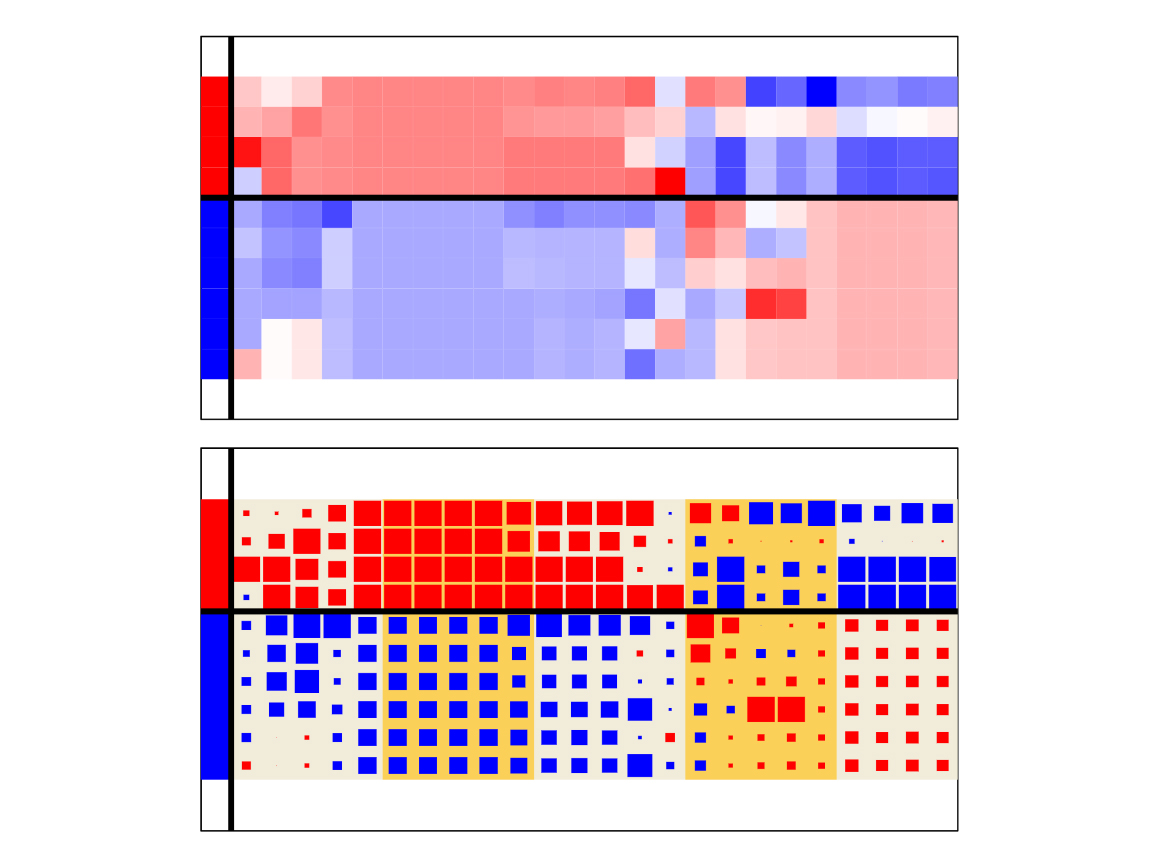
\includegraphics[width=1\linewidth]{ch-visualizer/figures/heatmap}
		\caption[Heat map versus association navigator]{\textit{Top:} A 
		traditional heat map. \textit{Bottom:} The association navigator on the 
		same set of data. 
		Each row corresponds to a pairwise scatter plot that was queried by the 
		VS and labeled by the user in 
		stage 1. The first column (to the left of the vertical black line) 
		denotes the user's label; as such, there is no size associated with the 
		characteristic. Red indicates ``not visually correlated'' 
		and blue indicates ``visually correlated''. The rest of the columns 
		corresponds to a different criterion of the associated pairwise 
		scatter plot (see Section~\ref{sec:visualizer:scatterplot}). Red 
		indicates a negative value while blue indicate a positive value. 		
		}
		\label{fig:visualizer:heatmap}
	\end{center}
\end{figure}
\bodyspacing

\noindent A classic heat map represents the qualities of each pair of variables 
as colors from a bivariate spectrum. 
Heat maps are difficult to interpret as they are 
one-dimensional; each end of the color spectrum represents minimum and maximum 
values respectively. It is unclear what the maximum or minimum values are 
because they depend on the domain of the whatever criterion the heat map is 
plotting; as such, the minimum may not necessarily be negative while the 
maximum may not necessarily be positive. Furthermore, the subtle variations in 
hue between colors make it difficult to compare the relative ranking of 
different variable pairs with similar colors. Buja \textit{et al.} 
propose an alternate, clearer method of visualizing the heat map, termed the 
``association navigator''~\cite{buja2016}. The association navigator is 
two-dimensional; the size of each field corresponds to the criterion's value 
while the color itself indicates if the criterion is positive or 
negative~\cite{buja2016}. As such, the 
association navigator only utilizes two colors rather than a spectrum of 
colors, making it simpler to distinguish between the two. By simplifying the 
color scheme and adding the dimension of size, the association navigator makes 
it easier to interpret and compare different pairs of data at a glance. 
The VS accommodates for both options, 
allowing the analyst method is preferred. 
With these visualizations of the active learning output, the user may better 
understand his/her own interests. 

\section{System output}
\label{sec:visualizer:plotgeneration:output}

After stage 2 is complete, there are three options for the system output. 
Two of them are concrete outputs 
that may be easily used in a final report on the data analysis findings, and 
the third is a refinement of the active learning component in stage 1.

\tablespacing
\begin{itemize}
	\item \textbf{Automatic plot generation:} The VS compiles a selection of 
	the most interesting and non-interesting plots along with their 
	associated transformation variables.
	
	\item \textbf{Graph comparison:} The VS accepts a numerical graph such as 
	$\hat{G}^{\text{num}}$, a correlation graph generated from one of the 
	numerical correlation coefficients described in 
	Section~\ref{sec:intro:correlation}, and measures the difference 
	between $\hat{G}^{\text{num}}$ and the visual graph $\hat{G}$ (the active 
	learning output). This is especially useful 
	for determining which numerical graph is ``closest'' to the visual graph, 
	allowing the user to select a more appropriate numerical method for their 
	analysis. Details on graph comparison methods and a similarity 
	selection strategy can be found in Chapter~\ref{ch:gc}.
	
	\item \textbf{Line-up test:} In the event that the classifier is not a 
	satisfactory representation of the analyst's interests, the VS may utilize 
	line-up tests to help determine where to query from further. Once the stage 
	1 component is refined and the classifier has been refit, the concrete 
	outputs mentioned above may then be generated if desired. For more 
	details on this methodology, see Section~\ref{sec:futurework:lineup}.
\end{itemize}
\bodyspacing

Because this thesis focuses on numerical and visual correlation graphs and 
their financial application, graph comparison is 
the most useful outputs from the visualization system. As such, it is one of 
our 
primary VS focuses. The next section provides a road map for the rest of this 
thesis, which focuses on two aspects of the VS. 